% Source: Code/ML_overlay/ir_rgb_registration/paper/ml_overlay_report_materials/ir_rgb_registration_report/figures/fig_parallax_depth_diagram.tex
\documentclass[tikz,border=10pt]{standalone}
\usepackage{tikz}
\usetikzlibrary{arrows.meta, calc}

\definecolor{Garnet}{RGB}{115, 0, 10}
\definecolor{Rose}{RGB}{204, 46, 64}
\definecolor{Atlantic}{RGB}{70, 106, 159}
\definecolor{Congaree}{RGB}{31, 65, 77}
\definecolor{Black70}{RGB}{92, 92, 92}

\begin{document}
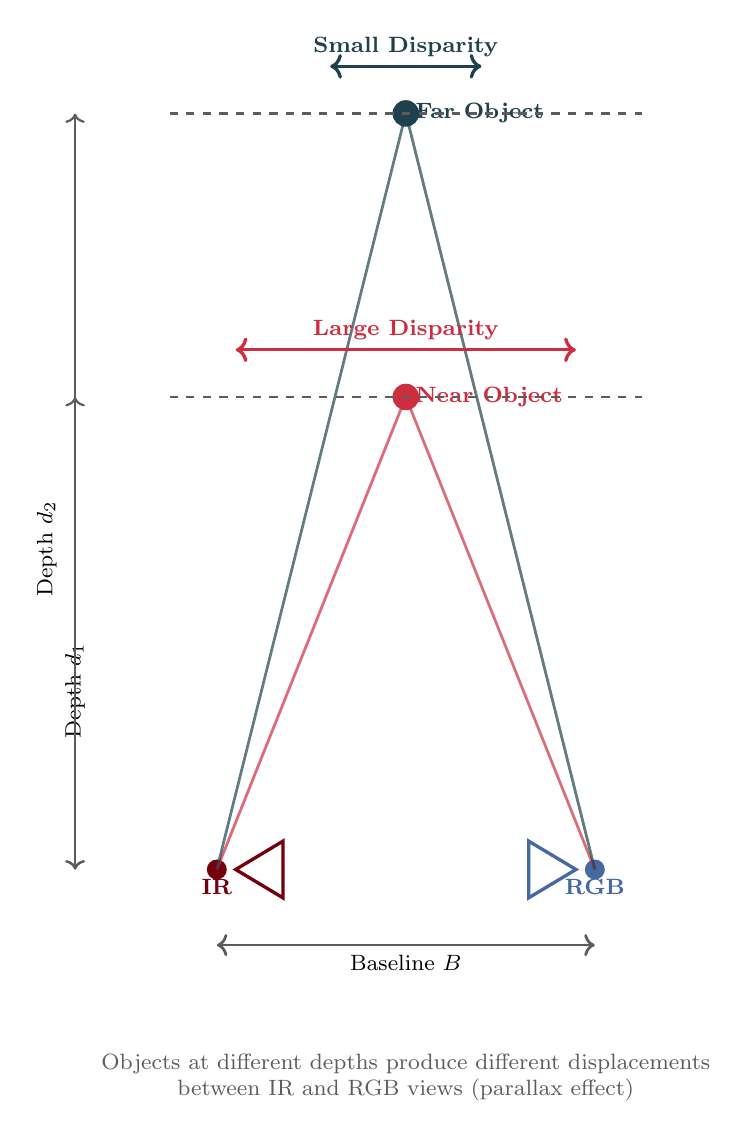
\begin{tikzpicture}[scale=1.2]

% Cameras at bottom
\coordinate (IR) at (0,0);
\coordinate (RGB) at (4,0);

% Camera bodies
\fill[Garnet] (IR) circle (3pt);
\draw[Garnet, line width=1.2pt] ($(IR)+(0.2,0)$) -- ++(0.5,0.3) -- ++(0,-0.6) -- cycle;
\node[below, font=\footnotesize\bfseries, Garnet] at (IR) {IR};

\fill[Atlantic] (RGB) circle (3pt);
\draw[Atlantic, line width=1.2pt] ($(RGB)+(-0.2,0)$) -- ++(-0.5,0.3) -- ++(0,-0.6) -- cycle;
\node[below, font=\footnotesize\bfseries, Atlantic] at (RGB) {RGB};

% Baseline
\draw[<->, Black70, line width=1pt] (0,-0.8) -- (4,-0.8);
\node[below, font=\footnotesize] at (2,-0.8) {Baseline $B$};

% Near object (higher up, closer)
\coordinate (Near) at (2,5);
\fill[Rose] (Near) circle (4pt);
\node[right, font=\footnotesize\bfseries, Rose] at (Near) {Near Object};

% Far object (higher up, farther)
\coordinate (Far) at (2,8);
\fill[Congaree] (Far) circle (4pt);
\node[right, font=\footnotesize\bfseries, Congaree] at (Far) {Far Object};

% Projection rays - Near object
\draw[Rose, line width=1pt, opacity=0.7] (IR) -- (Near);
\draw[Rose, line width=1pt, opacity=0.7] (RGB) -- (Near);

% Projection rays - Far object
\draw[Congaree, line width=1pt, opacity=0.7] (IR) -- (Far);
\draw[Congaree, line width=1pt, opacity=0.7] (RGB) -- (Far);

% Depth annotations
\draw[<->, Black70, line width=0.8pt] (-1.5,0) -- (-1.5,5);
\node[left, font=\footnotesize, rotate=90] at (-1.5,2.5) {Depth $d_1$};

\draw[<->, Black70, line width=0.8pt] (-1.5,0) -- (-1.5,8);
\node[left, font=\footnotesize, rotate=90] at (-1.8,4) {Depth $d_2$};

% Disparity illustration (image plane projections)
\draw[Black70, line width=0.8pt, dashed] (-0.5,5) -- (4.5,5);
\draw[Black70, line width=0.8pt, dashed] (-0.5,8) -- (4.5,8);

% Disparity annotation for near object
\draw[<->, Rose, line width=1.2pt] (0.2,5.5) -- (3.8,5.5);
\node[above, font=\footnotesize\bfseries, Rose] at (2,5.5) {Large Disparity};

% Disparity annotation for far object
\draw[<->, Congaree, line width=1.2pt] (1.2,8.5) -- (2.8,8.5);
\node[above, font=\footnotesize\bfseries, Congaree] at (2,8.5) {Small Disparity};

% Explanation text
\node[align=center, font=\footnotesize, Black70] at (2,-2.2) {
    Objects at different depths produce different displacements\\
    between IR and RGB views (parallax effect)
};

\end{tikzpicture}
\end{document}
